\documentclass[biblatexieee]{kclthesis}

\title{Argument Mining on Social Media}
\author{Danielius Marciukovas}
\modulecode{7CCSMPRJ}
\department{Department of Informatics}
\submissiontitle{Individual Project Submission 2018/19}
\studentnumber{1844311}
\emailaddress{danielius.marciukovas@kcl.ac.uk}
\programme{MSc Web Intelligence}
\supervisor{Josh Murphy}
\wordcount{3903}

\makenomenclature
\makeglossaries

\begin{document}
    \pagenumbering{gobble}
    
    \maketitle
    % \newpage
% \thispagestyle{empty}
% \mbox{}
% \newpage
    % \section*{Abstract}
Lorem ipsum dolor sit amet, consetetur sadipscing elitr, sed diam nonumy eirmod tempor invidunt ut labore et dolore magna aliquyam erat, sed diam voluptua. At vero eos et accusam et justo duo dolores et ea rebum. Stet clita kasd gubergren, no sea takimata sanctus est Lorem ipsum dolor sit amet. Lorem ipsum dolor sit amet, consetetur sadipscing elitr, sed diam nonumy eirmod tempor invidunt ut labore et dolore magna aliquyam erat, sed diam voluptua. At vero eos et accusam et justo duo dolores et ea rebum. Stet clita kasd gubergren, no sea takimata sanctus est Lorem ipsum dolor sit amet. 
    \pagenumbering{roman}
\setcounter{tocdepth}{4}
\tableofcontents
\newpage
    \thispagestyle{empty}
\listoffigures
\listoftables
\lstlistoflistings
\newpage
    % \mbox{}\newline\vspace{10mm} \mbox{}\LARGE
%
{\bf Acknowledgements} \normalsize \vspace{5mm}

I would like to thank my supervisor for providing me valuable support and feedback all throughout the year since I met him. He was helpful in guiding me in the right direction when I needed it and able to provide clearance on any matter whenever I had any concerns or questions. 

    \fancyhead{}
    \fancyfoot{}
    \pagestyle{fancy} 
    \fancyhead[R,L]{\sffamily\small \thepage}
    \fancyhead[LO]{\sffamily\small \nouppercase{\rightmark}}
    
    % \fancyhead[RO,L]{\sffamily\small \thepage}
    % \fancyhead[LO,RE]{\sffamily\small \nouppercase{\rightmark}}
    \renewcommand{\headrulewidth}{0.4pt}
    \renewcommand{\footrulewidth}{0.0pt}
    
    \pagenumbering{arabic}
    \section{Introduction}
\subsection{Overview} 
 Argumentation is a subject that studies processes involved in reasoning and the structure of reason itself. It is a field that encompasses and spans across multiple other fields, most notably language, philosophy, psychology, logic and has recently transcended into \gls{ai}. This is because \gls{ai} provides the ability to conjoin mental reasoning models and mathematical models for automated reasoning \citep{Lippi2016ArgumentationMS}. The applications of argument models within computer science and \gls{ai} are vast in possibilities. The ability to view and model such arguments provides important insight into how humans reason about different claims, how the claims are supported or disagreed with. Given an argument model applied to a discussion forum or a debate, this would provide an opportunity to understand more deeply and extract points of view that carry the most weight \citep{Cocarascu2017MiningBA}. Subsequently, it would be possible to analyse the flow of the discussion and see how the positions taken within the debate change over time as new arguments are introduced. On the other hand, same argument models can also allow us to investigate how a certain perception of something (review, feedback, etc.) can be altered \citep{ApproxToTruth}. Also, this is a hot topic with regards to ethics within the \gls{ai} system. The decisions that we delegate to \gls{ai} to make, have to be verifiable, thus meaning the system has to be able to show the arguments that it worked with and how the consensus on the decision was made. All in all, industries that would benefit would be law, politics and political debates, reviews and marketing, social media platforms to name a few.
 
\subsection{Argument Mining}
 
 \gls{am} is an intensive research field focused on automatically extracting arguments and their interrelationships from text documents. Due to recent technological advancements in other fields such as \gls{ai}, \gls{nlp} and \gls{ml}, this is becoming more and more possible. Moreover, internet provides unlimited amounts of data to analyse and extract arguments from with accessibility to websites such as Facebook, Twitter, Wikipedia Talks, Reddit and other popular social media pages 
 
 Unfortunately, this is not easy to do. The definition of argument is hard to express in mathematical or computer science terms. First of all, there are no limits as to how long an argument should be. An argument, depending on the corpora, can be a part of a sentence or the whole document could be one big argument backed by many smaller arguments within it (e.g. a certain law article is broken down into sections, which are then broken down into paragraphs and so on). Secondly, the nature of the argument has to be understood, to determine whether it is supporting any other argument, or attacking it. An argument is considered to be a supporting argument if it is on point with the view made by the previous original argument. Conversely, going back to the law example, an attack to the argument could be considered in the sense of an exception that is stated within the law, where the law doesn't apply. 
 
 These points coupled together mean that argument classification problem is dependent on meaning of the argument itself, which makes this also a \gls{nlp} problem. Context or topic of the corpora matters a lot as well, because of language stylistic differences. It is no surprise that legal documents entail a more precise syntactical text structure, due to the nature of the industry requiring concrete descriptions to cover and exclude very specific cases of application. On the other hand, texts found in social media are of a more diverse linguistic composition, where messages posted by users can be very conversational or carry a meaning that is only understood by a certain group of people (e.g. abbreviations, specific background required).

\subsection{Project Aims and Objectives} 
 The aim of this project is to gain an up to date knowledge of current trends and advancements within the field of argumentation mining, to create a tool that given a specific chain of arguments in text form would analyse such arguments and construct an \gls{af} displaying the winning or most convincing arguments, and to contribute to the research community by explaining views and sharing ideas pertaining to the problem at hand.

\subsection{Background and Literature Survey} \label{sub:background}

This part is for literature review.

% It gives an overall picture about the work with a clear review of the relevant literature.  The background of the project should be given.  What have been done to deal with the problem should be stated clearly.  The pros and cons of various existing algorithms and approaches should be stated as well.  Differences between your proposed method and the existing ones should be briefly described. 

%The following links may help on the literature review: IEEE Xplore digital library: a resource for accessing IEEE published scientific and technical publications. (You must be with King's network to get access to the digital library) ScienceDirect.com: an electronic database offering journal papers not published by IEEE (You must be with King's network to get access to the database)

    \section{Background Theories} 

This section describes what the reader has to know in order to understand my project.
    \section{Literature Review}
    \subsection{Overview}
        In \autocite{Lippi2016ArgumentationMS}, the authors focus on giving the reader a broad overview of argumentation and various computational challenges associated with it. Authors proceed to entertain the thoughts of what the breakthrough by solving these challenges would mean on a societal level and the impact of it. Moving on, the paper also describes different approaches that were previously experimented within the domains of argumentation and \gls{am}, mainly extracting arguments from unstructured text, which authors consider to be the core \gls{am} task. The core \gls{am} tasks are explained sufficiently for the reader to understand the differences between them. On the other hand, authors give only brief mentions to other \gls{am} tasks (opinionated claim analysis, premise verification, etc.), without giving a clear description of how they are different from each other. Also, the article does not provide any concrete evaluation of each methods, which makes it hard to gauge which approach has been the most successful so far or what the results were. Overall, the authors give a good overview of active research topics and different directions that the domain has taken.
        
    \subsection{Textual Entailment}
        \gls{te} is one of the most popular approaches to identify argument \textit{attack} and \textit{support} relationships. The \autocite{Cabrio2012NaturalLA, Cabrio2012CombiningTE} papers give a general introduction to using \gls{te} as a means for identifying how one argument stands in relation to the other. Authors make a strong assumption that \textit{support} relation in \gls{baf} is the same as \textit{entailment} in \gls{te} and \textit{attack} in \gls{baf} is as \textit{contradiction} in \gls{te}. They test this theory on a set of arguments gathered from Debatepedia, an online debate forum where users express pros and cons on various topics. The language used at such discussions is quite different from loose and unstructured linguistics that can be seen in online social media corpus, which makes it hard to predict how the approach would do given a unpredictable environment. The system used for deciding if there exists a relation is called \gls{edits}, which states that the entailment relation probability of two arguments in a pair is greater the lower the number of changes need to be made between those two arguments, and vice versa. The chosen argument pair set is small, only 200 (100 used as a training set and 100 as test set), which is arguably insufficient to accurately assess the proposed approach, nevertheless, authors managed to accurately compute argument interrelations 75\% of the time, which is better than expected. In \autocite{Cabrio2013ANL, Cabrio2013DetectingBS}, the same authors have improved upon their research by exploring the \textit{support}-\textit{entailment} relationship, mostly by taking a step back on their previous assumption. The authors give an overview of semantic inferences in \gls{nlp}, in the sense that it is not always the case that an argument that supports another argument necessarily entails the latter argument in context. This was done by introducing a third labelling of argument pairs as \textit{null}, when such relation cannot be determined just from looking at those two arguments. Subsequently, same approach was applied to attacks, mainly by introducing 4 different types of complex attacks (\textit{supported}, \textit{mediated}, \textit{secondary}, \textit{extended}). The idea is similar, in that not all \textit{attacks} are \textit{contradictions}, thus making this case more subtle in general, requiring additional specification to identify attack relations. The results show that approximately 60\% of support argument pairs - \gls{te} holds; and for attacks - contradiction is present in about 70\% of argument pairs.
     
        Recently, the research in \gls{am} has taken a turn to social media, namely Twitter. Twitter is different from Debatepedia in that it often contains noisy, unstructured messages. This is mostly because of the specific restriction that Twitter imposes, being 140 character limit, which forces the user to express thoughts in short. Twitter is a good choice, because it provides open \gls{api} and it is possible to filter messages based on specific topics, that are defined with the use of a hashtag symbol (\#). In \autocite{Bosc2016DARTAD}, the authors describe their methodology for classifying tweets as argumentative or non-argumentative. The methodology provides extensive description of how to treat different types of tweets, how to evaluate the substance of each tweet and shows relevant examples. A further study \autocite{Bosc2016TweetiesSP} by the same authors put such dataset to practice. The paper divides the work into 4 major steps that have to be taken from start to finish and discusses different approaches within each of those steps. The steps are as follows: \textit{1)} tweets need to be separated into two pools - either argumentative or non-argumentative; \textit{2)} argumentative tweets need to be further divided into separate groups by topic, and then, argument pairs have to be created; \textit{3)} argument relationship within the argument pairs have to be predicted as either \textit{attack} or \textit{support}; \textit{4)} argumentation graph has to be built. First and second tasks are trivial compared to the third one, as is evident based on views expressed in the paper. Different approaches were tested while tackling the third task, \gls{eop}, \gls{te}, neural sequence classifiers, though all with unsatisfying results, accuracies being less than 20\%.
     
    \subsection{Other Approaches}
        Here are briefly described other methods that were taken to extract arguments from unstructured texts:
        \begin{itemize}
            \item The \autocite{Cocarascu2017IdentifyingAA} paper uses Deep Learning and Long-Short Term Memory unidirectional and bidirectional networks to classify relations as either \textit{attack}, \textit{support} or \textit{neither support nor attack} and achieved an accuracy of 89.53\%. 
            
            \item In \autocite{Cocarascu2017MiningBA} the authors employ a methodology that tries to discover argument relations by grouping arguments into groups of similar topics. They showcase this by using an example containing hotel reviews, with reviews being grouped into 6 different topics. Also, the paper gives a brief description of how each topic could be given a strength score based on existing arguments.
            
            \item The \autocite{ApproxToTruth} paper analyses how a part of online comment network relates to the whole network in terms of acceptable conclusions drawn. In other words, by reading through an online debate, how similar conclusions can be drawn at that point in time compared to the overall consensus of the debate taking into equation all existing arguments. This is done by comparing grounded extensions of the two argumentation frameworks.
            
            \item The \autocite{Cocarascu2016DetectingDR} gives a \gls{ml} approach to detecting deceptive reviews by constructing topic independent \gls{aaf} and topic dependent \gls{baf}. Several algorithms (Random Forests, Logistic Regression, Na{\"i}ve Bayes) are used to evaluate the performances.
            
            \item In \autocite{Dusmanu2017ArgumentMO} supervised classification algorithms are used to detect arguments on Twitter. Authors also propose new avenues for research, namely facts recognition and source identification with regards to arguments.
            
            \item In \autocite{Lippi2015ContextIndependentCD}, the authors provide a context independent (topic independent) methodology for automatically extracting argument frameworks from unstructured text. They do this by splitting text into sentences and for each sentence building tree structures representing syntactical components of a sentence. The results are quite satisfactory with 74.6\%/68.4\% of precision/recall performances.
        \end{itemize}
    \section{Schedule and Planning}
    \begin{table}[!htbp]
    \centering
    \begin{tabular}{|l|c|c|c|c|c|c|c|c|c|c|c|c|c|c|c|c|}
        \toprule
        & \multicolumn{4}{c|}{May} & \multicolumn{4}{c|}{June} & \multicolumn{4}{c|}{July} & \multicolumn{4}{c|}{August} \\ 
        \midrule
        
        Research Code Libraries & \multicolumn{2}{c|}{\cellcolor{brown}} & & & & & & & & & & & & & & \\
        \hline
        Web Scraper Implementation & & & \multicolumn{2}{c|}{\cellcolor{blue}} & & & & & & & & & & & & \\
        \hline
        
        Social Media Data Mining & & & & & \multicolumn{3}{c|}{\cellcolor{orange}} & & & & & & & & & \\
        \hline
        
        Implementation of \gls{te} Algorithms & & & & & & & & \multicolumn{2}{c|}{\cellcolor{green}} & & & & & & & \\
        \hline
        
        Evaluation of \gls{te} Algorithms & & & & & & & & & & \cellcolor{red} & & & & & & \\
        \hline
        
        Implementation of \gls{af} & & & & & & & & & & & \multicolumn{2}{c|}{\cellcolor{gray}} & & & & \\
        \hline
        
        Overall System Testing & & & & & & & & & & & & & \cellcolor{yellow} & & & \\
        \hline
        
        Conclusion, Presentation, Future Work & & & & & & & & & & & & & & \multicolumn{2}{c|}{\cellcolor{purple}} & \\
        \bottomrule
    \end{tabular}
    \caption{Proposed timetable for MSc Individual Project}
    \label{table:timetable}
\end{table}
    
    Short description of each goal:
    \begin{itemize}
        \item Research Code Libraries - analysing existing code libraries and frameworks, making a choice on programming language, etc.
        \item Web Scraper - decide on a mechanism of extracting text/arguments from social media, whether that's a manually coded web scraper or access to \gls{api} if there is one.
        \item Social Media Data Mining - transforming raw text into data structures for future \gls{te} algorithm use.
        \item Implementation of \gls{te} Algorithms - implementing the \gls{te} algorithm with specific properties/parameters that suit the project.
        \item Evaluation of \gls{te} Algorithms - testing and evaluating the results of the algorithms implemented.
        \item Implementation of \gls{af} - using the results of \gls{te} algorithm to build \gls{af}.
        \item Overall System Testing - putting everything together into a coherent project.
        \item Conclusion, Presentation, Future Work - drawing appropriate conclusions of the project, proposing future work areas or possible improvements, creating presentation slides, other finishing works.
    \end{itemize}
    \section{Main Result}
The chapter reports the contribution of your work.  For example, it could contain the following sub-sections to summarise the contribution of the project: Theoretical Development, Analysis and Design, Implementation and Experimental Work, Results, Observation and Discussion.

\subsection{Maths}
\begin{equation}\label{eq:BS}
\frac{\D S_t}{S_t} = r \D t + \sigma \D W_t,
\qquad S_0>0,
\end{equation}

The equation $\sigma = m a$ follows easily~\cite{Doe11}.


\subsection{Glossary and acronyms}

\Glspl{Linux} and other Unix operating systems are better then Windows because they support \gls{lvm} out of the box~\cite{Joh11}\insertref{A ref is missing here}. 

\subsection{Figures}
Here is an example~\cite{JohSil05} of how to inserta picture:

\begin{figure}[!ht]
\centering
\subfigure{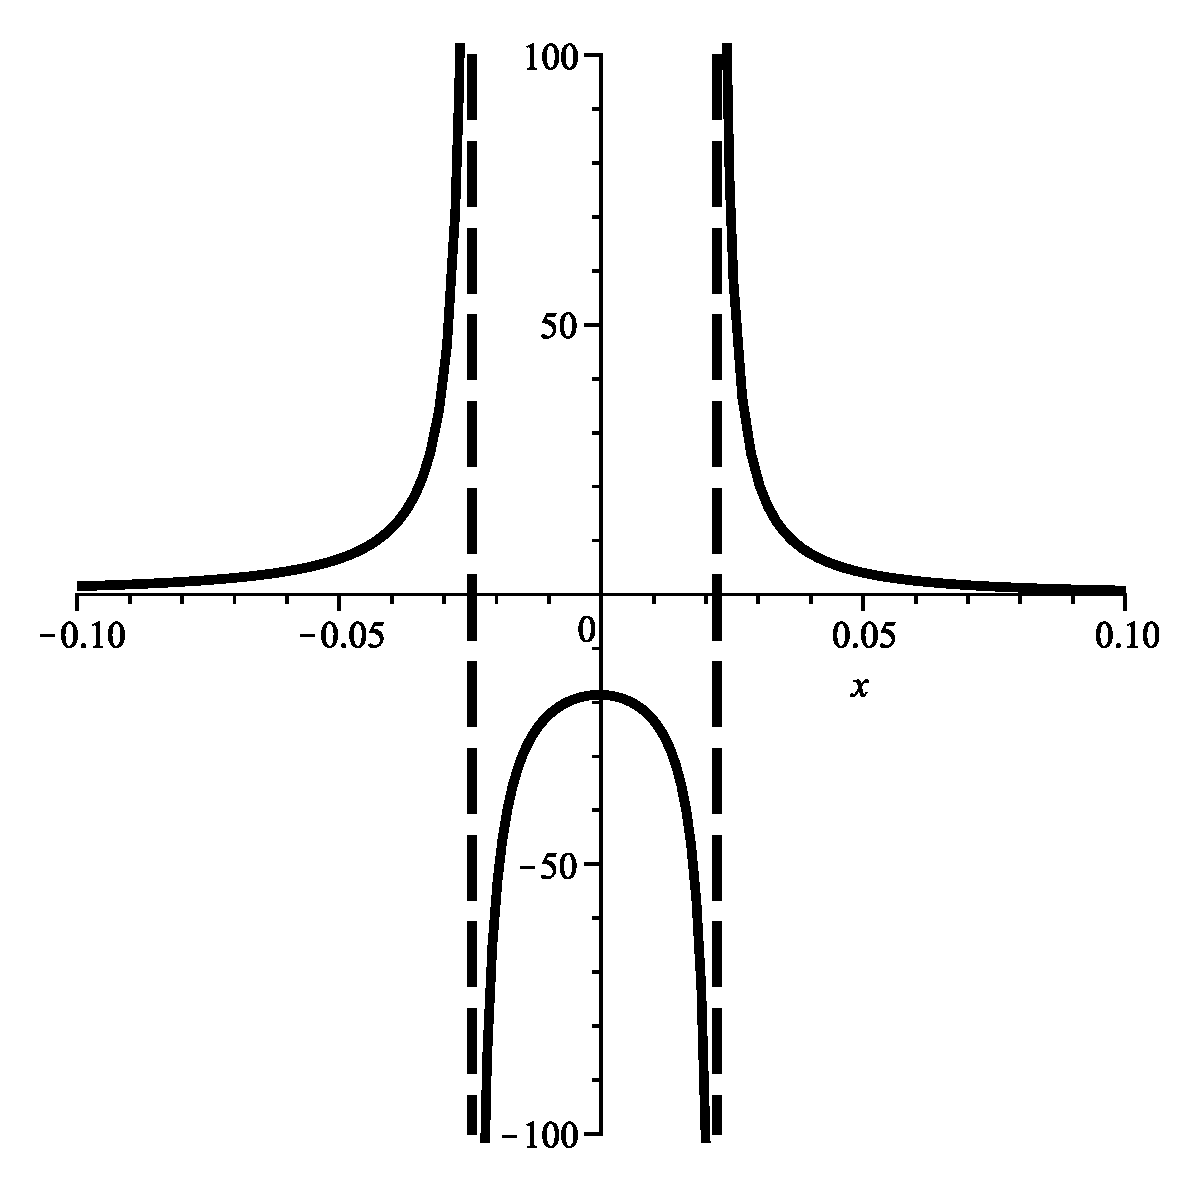
\includegraphics[scale=0.2]{figures/Picture.eps}}
\caption{This is the caption for the figure.}
\label{fig:Pict}
\end{figure}


\begin{figure}[!ht]
\centering
\missingfigure{If you know there will be a figure, but you still need to create it.}
\caption{This is the caption for the figure which is not even present.}
\label{fig:PictMis}
\end{figure}


Lorem ipsum dolor sit amet, consetetur sadipscing elitr, sed diam nonumy eirmod tempor invidunt ut labore et dolore magna aliquyam erat, sed diam voluptua. At vero eos et accusam et justo duo dolores et ea rebum. Stet clita kasd gubergren, no sea takimata sanctus est Lorem ipsum dolor sit amet. Lorem ipsum dolor sit amet, consetetur sadipscing elitr, sed diam nonumy eirmod tempor invidunt ut labore et dolore magna aliquyam erat, sed diam voluptua. At vero eos et accusam et justo duo dolores et ea rebum. Stet clita kasd gubergren, no sea takimata sanctus est Lorem ipsum dolor sit amet.\todo{This is a small Todo, please take care!}

or two side-by-side pictures:

\begin{figure}[!ht]
\centering
\subfigure{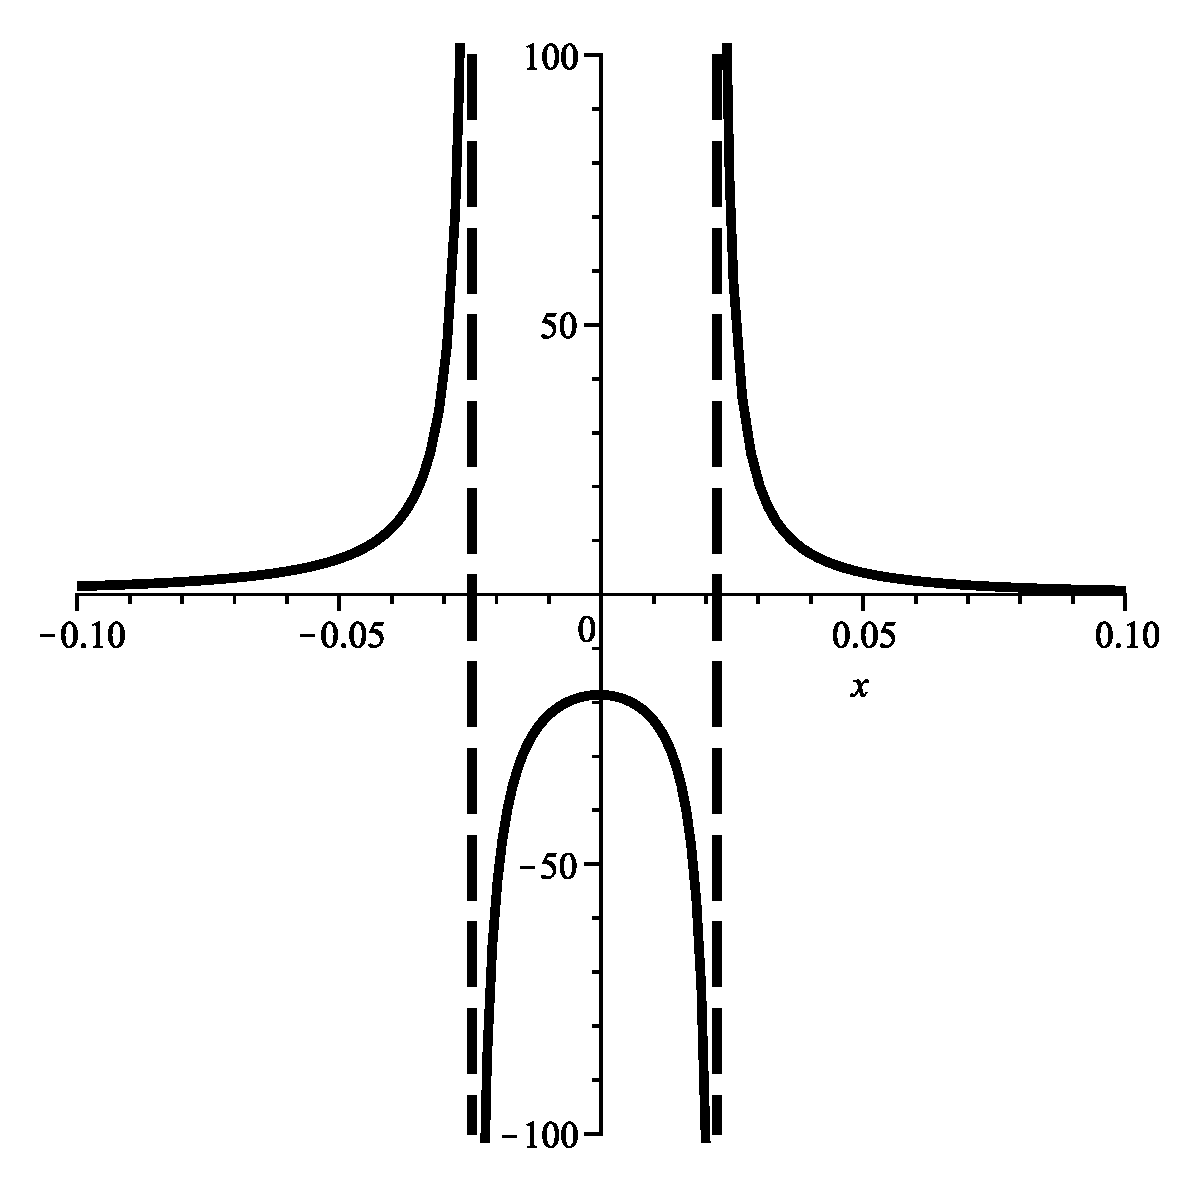
\includegraphics[scale=0.3]{figures/Picture.eps}}
\hspace{15pt}
\subfigure{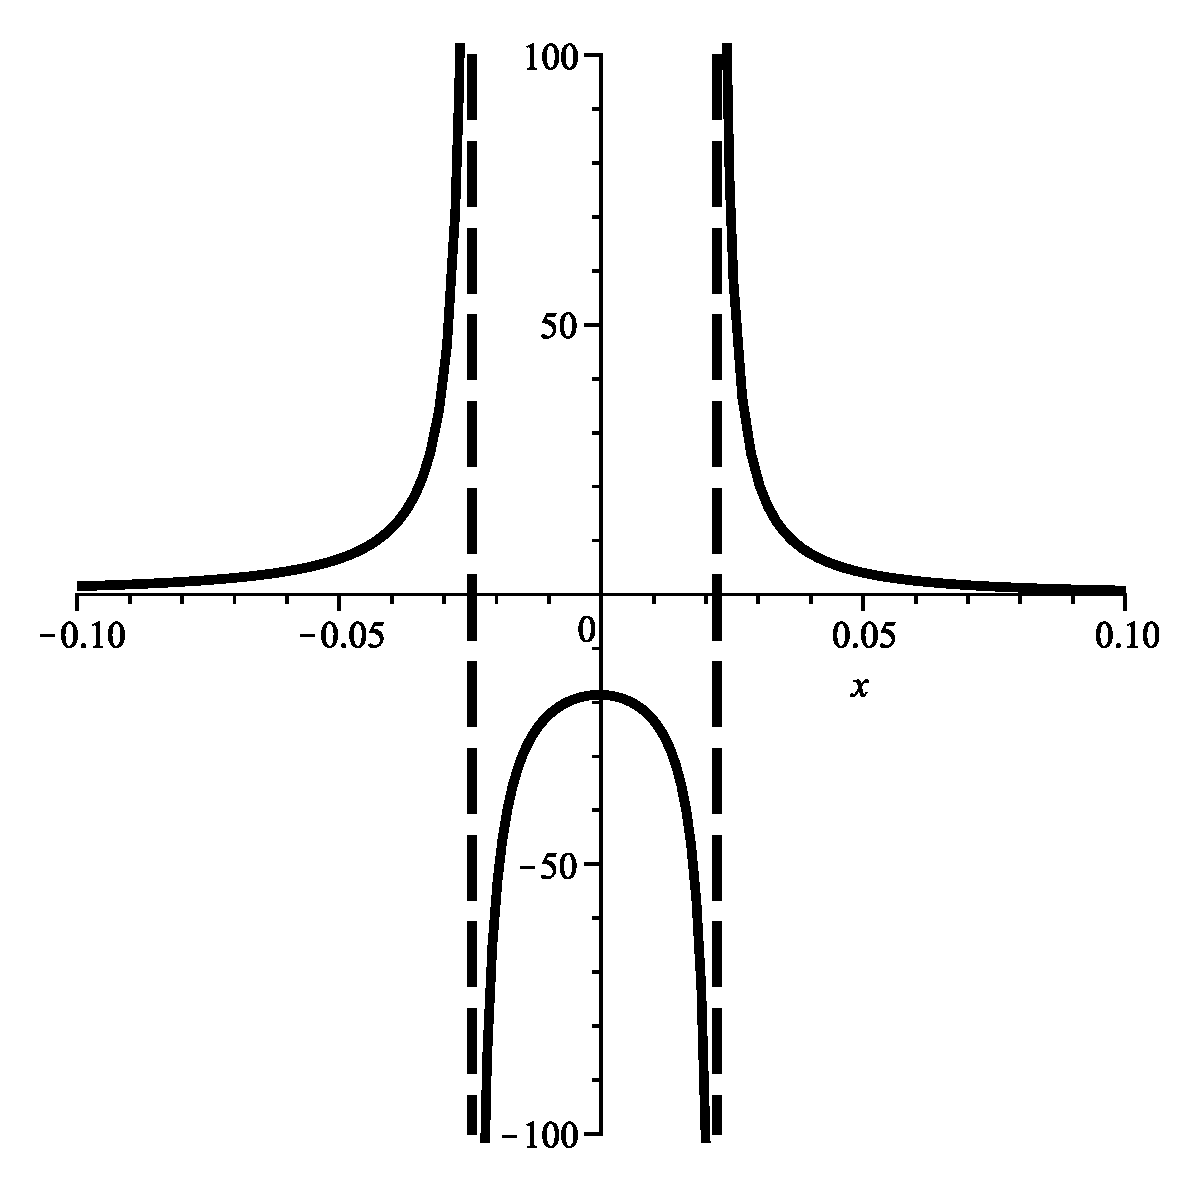
\includegraphics[scale=0.3]{figures/Picture.eps}}

\caption{Another caption}
\label{fig:Pict2}
\end{figure}



\subsection{Table}
Lorem ipsum dolor sit amet, consetetur sadipscing elitr, sed diam nonumy eirmod tempor invidunt ut labore et dolore magna aliquyam erat, sed diam voluptua. At vero eos et accusam et justo duo dolores et ea rebum. Stet clita kasd gubergren, no sea takimata sanctus est Lorem ipsum dolor sit amet. Lorem ipsum dolor sit amet, consetetur sadipscing elitr, sed diam nonumy eirmod tempor invidunt ut labore et dolore magna aliquyam erat, sed diam voluptua. At vero eos et accusam et justo duo dolores et ea rebum. Stet clita kasd gubergren, no sea takimata sanctus est Lorem ipsum dolor sit amet\explainindetail{This needs further explanation}.
\begin{table}[!ht]
	\centering
	\begin{tabular}{|l|rl|}
		\hline
		Something & Someother & Thing \\
  		Seems & to be & good\\
  		\hline
  	\end{tabular}
  	\caption{Random data for a table.}
\end{table}

Lorem ipsum dolor sit amet, consetetur sadipscing elitr, sed diam nonumy eirmod tempor invidunt ut labore et dolore magna aliquyam erat, sed diam voluptua. At vero eos et accusam et justo duo dolores et ea rebum. Stet clita kasd gubergren, no sea takimata sanctus est Lorem ipsum dolor sit amet. Lorem ipsum dolor sit amet, consetetur sadipscing elitr, sed diam nonumy eirmod tempor invidunt ut labore et dolore magna aliquyam erat, sed diam voluptua. At vero eos et accusam et justo duo dolores et ea rebum. Stet clita kasd gubergren, no sea takimata sanctus est Lorem ipsum dolor sit amet.


\section{Model calibration}
\subsection{What is calibration?}
Here is an example of a matrix\cite{website:fermentas-lambda} in $A\in\mathcal{M}_n(\RR)$:
$$
A = 
\begin{pmatrix}
a_{11} & a_{12} & \ldots & a_{1n}\\
a_{21} & \ddots & \ddots  & \vdots\\
\vdots &  \ddots & \ddots  & \vdots\\
a_{n1} &  \ldots &  \ldots & a_{1n}.
\end{pmatrix}
$$

\subsection{Numerical methods for calibration}
...



    % \section{Conclusion} \label{conclusions}
    This section briefly summarises what has been achieved throughout the project. Analysis performed on two government systems used by English speaking countries showcase interesting social tendencies how the public treats and reacts to opposing parties. It is sufficient to say that this is only the tip of the iceberg and there are many different topics that can be explored in the same manner, not only politics as was chosen here.
    
    The contribution to research community is substantial. The trained classifier is in line with expected performance given the circumstances of hardware limitations, and the overall software is a stepping stone to combining argument mining, extraction, relation detection and framework analysis into one coherent process, with high hopes of becoming an advanced system capable of handling multiple models and multiple social media platforms.
    \newpage

\newacronym{ai}{AI}{Artificial Intelligence}
\newacronym{nlp}{NLP}{Natural Language Processing}
\newacronym{ml}{ML}{Machine Learning}
\newacronym{te}{TE}{Textual Entailment}
\newacronym{af}{AF}{Argumentation Framework}
\newacronym{aaf}{AAF}{Abstract Argumentation Framework}
\newacronym{baf}{BAF}{Bipolar Argumentation Framework}
\newacronym{am}{AM}{Argumentation Mining}
\newacronym{edits}{EDITS}{Edit Distance Textual Entailment Suite}
\newacronym{api}{API}{Application Programming Interface}
\newacronym{eop}{EOP}{Excitement Open Platform}
\newacronym{rnn}{RNN}{Recurrent Neural Network}
\newacronym{lstm}{LSTM}{Long Short-Term Memory}
\newacronym{snli}{SNLI}{Stanford Natural Language Inference}
\newacronym{ram}{RAM}{Rapid-Access Memory}
\newacronym{cpu}{CPU}{Central Processing Unit}
\newacronym{gpu}{GPU}{Graphics Processing Unit}
\newacronym{vram}{VRAM}{Video Rapid-Access Memory}
\newacronym{csv}{CSV}{Comma-Separated Values}
\newacronym{os}{OS}{Operating System}
\newacronym{glove}{GloVe}{Global Vectors for Word Representation}
\newacronym{ddos}{DDoS}{Distributed Denial of Service}
\newacronym{url}{URL}{Uniform Resource Locator}
%\newglossaryentry{pi}{name={\ensuremath{\pi}}, description={ratio of circumference of circle to its diameter}, sort=pi}
%\newglossaryentry{Linux}{name=Linux,description={is a generic term referring to the family of Unix-like computer operating systems that use the Linux kernel}, plural=Linuces}
\printglossaries

\newpage
    
    %%%%% References
    % \nocite{*}
    
    % For KCL Harvard V1: \bibliographystyle{kclharvardv1}
    % For natbib-ieee: 
    % \bibliographystyle{ieeetr}
    % \bibliography{bibs/bibliography}
    % For biblatex-ieee:
    \printbibliography
    
    %%%%% Declaration
    % %\thispagestyle{empty}


\mbox{}\newline\vspace{10mm} \mbox{}\LARGE
%
{\bf Declaration} \normalsize \vspace{5mm}

I declare that this thesis is the solely effort of the author.
I did not use any other sources and references than the listed ones. I have marked all contained direct or indirect statements from other sources as such.

Neither this work nor significant parts of it were part of another review process.
I did not publish this work partially or completely yet.
The electronic copy is consistent with all submitted copies.

\bigskip
\bigskip
\bigskip
\bigskip


Signature and date: 





    
    %%%%% Appendix 
    % \appendix
    % \section{Schedule and Planning} \label{apx_A}
    \begin{table}[!htbp]
    \centering
    \begin{tabular}{|l|c|c|c|c|c|c|c|c|c|c|c|c|c|c|c|c|}
        \toprule
        & \multicolumn{4}{c|}{May} & \multicolumn{4}{c|}{June} & \multicolumn{4}{c|}{July} & \multicolumn{4}{c|}{August} \\ 
        \midrule
        
        Research Code Libraries & \multicolumn{2}{c|}{\cellcolor{brown}} & & & & & & & & & & & & & & \\
        \hline
        Web Scraper Implementation & & & \multicolumn{2}{c|}{\cellcolor{blue}} & & & & & & & & & & & & \\
        \hline
        
        Social Media Data Mining & & & & & \multicolumn{3}{c|}{\cellcolor{orange}} & & & & & & & & & \\
        \hline
        
        Implementation of \gls{te} Algorithms & & & & & & & & \multicolumn{2}{c|}{\cellcolor{green}} & & & & & & & \\
        \hline
        
        Evaluation of \gls{te} Algorithms & & & & & & & & & & \cellcolor{red} & & & & & & \\
        \hline
        
        Implementation of \gls{af} & & & & & & & & & & & \multicolumn{2}{c|}{\cellcolor{gray}} & & & & \\
        \hline
        
        Overall System Testing & & & & & & & & & & & & & \cellcolor{yellow} & & & \\
        \hline
        
        Conclusion, Presentation, Future Work & & & & & & & & & & & & & & \multicolumn{2}{c|}{\cellcolor{purple}} & \\
        \bottomrule
    \end{tabular}
    \caption{Proposed timetable for MSc Individual Project}
    \label{table:timetable}
\end{table}
    
    Short description of each goal:
    \begin{itemize}
        \item Research Code Libraries - analysing existing code libraries and frameworks, making a choice on programming language, etc.
        \item Web Scraper - decide on a mechanism of extracting text/arguments from social media, whether that's a manually coded web scraper or access to \gls{api} if there is one.
        \item Social Media Data Mining - transforming raw text into data structures for future \gls{te} algorithm use.
        \item Implementation of \gls{te} Algorithms - implementing the \gls{te} algorithm with specific properties/parameters that suit the project.
        \item Evaluation of \gls{te} Algorithms - testing and evaluating the results of the algorithms implemented.
        \item Implementation of \gls{af} - using the results of \gls{te} algorithm to build \gls{af}.
        \item Overall System Testing - putting everything together into a coherent project and performing overall evaluation.
        \item Conclusion, Presentation, Future Work - drawing appropriate conclusions of the project, proposing future work areas or possible improvements, creating presentation slides, other finishing works.
    \end{itemize}


\end{document}
